% Template baseado no arquivo default:
% /usr/lib/R/site-library/rmarkdown/rmd/latex/default-1.17.0.2.tex

\documentclass[a4paper,]{book}
\usepackage{lmodern}
\usepackage{amssymb,amsmath}
\usepackage{ifxetex,ifluatex}
\usepackage{fixltx2e} % provides \textsubscript
\ifnum 0\ifxetex 1\fi\ifluatex 1\fi=0 % if pdftex
  \usepackage[T1]{fontenc}
  \usepackage[utf8]{inputenc}
\else % if luatex or xelatex
  \ifxetex
    \usepackage{mathspec}
  \else
    \usepackage{fontspec}
  \fi
  \defaultfontfeatures{Ligatures=TeX,Scale=MatchLowercase}
\fi
% use upquote if available, for straight quotes in verbatim environments
\IfFileExists{upquote.sty}{\usepackage{upquote}}{}
% use microtype if available
\IfFileExists{microtype.sty}{%
\usepackage{microtype}
\UseMicrotypeSet[protrusion]{basicmath} % disable protrusion for tt fonts
}{}
\usepackage[inner = 4cm,outer = 3cm,top = 3cm,bottom = 3cm]{geometry}
\usepackage{hyperref}
\PassOptionsToPackage{usenames,dvipsnames}{color} % color is loaded by hyperref
\hypersetup{unicode=true,
            pdftitle={epidemioR: Epidemiologia de Doenças de Plantas Aplicada com R},
            colorlinks=true,
            linkcolor=green,
            citecolor=blue,
            urlcolor=blue,
            breaklinks=true}
\urlstyle{same}  % don't use monospace font for urls
\usepackage{natbib}
   \bibpunct{(}{)}{;}{a}{,}{,}       % opções que definem estilo
   \setlength{\bibhang}{0em}         % indentação da referência
   \setlength{\bibsep}{2em}          % espaçamento vertical entre as citações
\bibliographystyle{./config/TESALQmod.bst}
\usepackage{longtable,booktabs}
\usepackage{graphicx,grffile}
\makeatletter
\def\maxwidth{\ifdim\Gin@nat@width>\linewidth\linewidth\else\Gin@nat@width\fi}
\def\maxheight{\ifdim\Gin@nat@height>\textheight\textheight\else\Gin@nat@height\fi}
\makeatother
% Scale images if necessary, so that they will not overflow the page
% margins by default, and it is still possible to overwrite the defaults
% using explicit options in \includegraphics[width, height, ...]{}
\setkeys{Gin}{width=\maxwidth,height=\maxheight,keepaspectratio}
\IfFileExists{parskip.sty}{%
\usepackage{parskip}
}{% else
\setlength{\parindent}{0pt}
\setlength{\parskip}{6pt plus 2pt minus 1pt}
}
\setlength{\emergencystretch}{3em}  % prevent overfull lines
\providecommand{\tightlist}{%
  \setlength{\itemsep}{0pt}\setlength{\parskip}{0pt}}
\setcounter{secnumdepth}{5}
% Redefines (sub)paragraphs to behave more like sections
\ifx\paragraph\undefined\else
\let\oldparagraph\paragraph
\renewcommand{\paragraph}[1]{\oldparagraph{#1}\mbox{}}
\fi
\ifx\subparagraph\undefined\else
\let\oldsubparagraph\subparagraph
\renewcommand{\subparagraph}[1]{\oldsubparagraph{#1}\mbox{}}
\fi
%---- config/preamble.tex ----------------------------------------------

\usepackage[brazil]{babel}
\usepackage{mathpazo}
\usepackage{eulervm}
\usepackage{inconsolata}
\urlstyle{tt}
%\usepackage[utf8]{inputenc}
%\usepackage[T1]{fontenc}
\usepackage{booktabs}
\usepackage{epigraph}
\usepackage{wallpaper}

% https://theoryl1.wordpress.com/2016/01/15/fontawesome-in-pdftex/
% http://linorg.usp.br/CTAN/fonts/fontawesome/doc/fontawesome.pdf
\usepackage{fontawesome}

%--------------------------------------------

\usepackage{fancyhdr}

% \pagestyle{fancy}
% \pagestyle{fancy}
% \addtolength{\headsep}{25pt}
\setlength{\headheight}{18pt}
% \setlength{\footheight}{24.0pt}
\fancyhead{}
% \fancyhead[LE,RO]{\thepage}
% \fancyhead[LE]{\footnotesize{\thepage \hfill \scshape\nouppercase{\leftmark}}}
\fancyhead[LE]{\footnotesize{\thepage \hfill \scshape\nouppercase{Capítulo \thechapter}}}
% \fancyhead[RE]{\scriptsize\leftmark}
% \fancyhead[RO]{\footnotesize{\scshape\nouppercase{\rightmark}} \hfill \thepage}
\fancyhead[RO]{\footnotesize{\thesection \hfill \thepage}}
% \fancyhead[LO]{\scriptsize\rightmark}
\fancyfoot{}
% \fancyfoot[RE, LO]{www.leg.ufpr.br/wpde2013}
\fancyfoot[LO]{\footnotesize{\textbf{epidemioR}: epidemiologia de doenças de plantas aplicada com R}}
\fancyfoot[LE]{{\footnotesize \it lemid.github.io/epidemioR}}
\renewcommand{\headrulewidth}{0.4pt}
\renewcommand{\footrulewidth}{0.4pt}

\usepackage[Lenny]{fncychap}
\ChNameVar{\Large}
\ChNumVar{\Huge\itshape}
\ChTitleVar{\huge}

\pagestyle{empty}
% TODO: definir '\pagestyle{fancy}' no Rmd do primeiro capítulo.
% ATTENTION: '\pagestyle{fancy}' está sendo adicionado pela função
% `author_chapters()` definida em `setup.R`.

%--------------------------------------------

\usepackage{makeidx}
\makeindex

\renewcommand{\labelitemi}{\raisebox{0.25ex}{\footnotesize $\blacktriangleright$}}
\renewcommand{\labelitemii}{\raisebox{0.25ex}{\footnotesize $\blacktriangleright$}}
\renewcommand{\labelitemiii}{\raisebox{0.25ex}{\footnotesize $\blacktriangleright$}}
\renewcommand{\labelitemiv}{\raisebox{0.25ex}{\footnotesize $\blacktriangleright$}}

\usepackage{indentfirst}
  \setlength{\parindent}{1.2cm}
\usepackage{setspace}
  \onehalfspace
%\renewcommand{\baselinestretch}{1.5}

%\usepackage[
%  %margin=0pt,
%  %width=1\linewidth,
%  %font=small,
%  %justification=center,
%  singlelinecheck=off,
%  %format=plain,
%  %labelfont=bf,
%  %textfont=normal,
%  %labelformat=simple,
%  %format=hang,
%  up]{caption}
%\captionsetup[table]{skip=0pt, justification=raggedright, singlelinecheck=off}
%\captionsetup[table]{skip=0pt, singlelinecheck=off}
%\LTcapwidth=5.65in

%---- config/preamble.tex ----------------------------------------------

\usepackage{pdfpages} % Incluir PDF da capa: \includepdf{mycover.pdf}.

%%% Use protect on footnotes to avoid problems with footnotes in titles
\let\rmarkdownfootnote\footnote%
\def\footnote{\protect\rmarkdownfootnote}

%%% Change title format to be more compact
\usepackage{titling}

% Create subtitle command for use in maketitle
\newcommand{\subtitle}[1]{
  \posttitle{
    \begin{center}\large#1\end{center}
    }
}

\setlength{\droptitle}{-2em}
  \title{epidemioR: Epidemiologia de Doenças de Plantas Aplicada com R}
  \pretitle{\vspace{\droptitle}\centering\huge}
  \posttitle{\par}

%~   %~ \author{true \\ true}
  %~ \preauthor{\centering\large\emph}
  %~ \postauthor{\par}
%~ 
% ---- Autores ----
\author{
      Walmes Marques Zeviani
  %~ \\ Departamento de Estatística · UFPR 
  %~ \\ \texttt{\href{mailto:walmes@ufpr.br}{\nolinkurl{walmes@ufpr.br}}} 
     \and\\
      Louise Larissa May De Mio
  %~ \\ Departamento de Fitotecnia e Fitossanidade · UFPR 
  %~ \\ \texttt{\href{mailto:maydemio@ufpr.br}{\nolinkurl{maydemio@ufpr.br}}} 
    }

  \predate{\centering\large\emph}
  \postdate{\par}
  \date{Última atualização em 08 de setembro de 2019}

\begin{document}

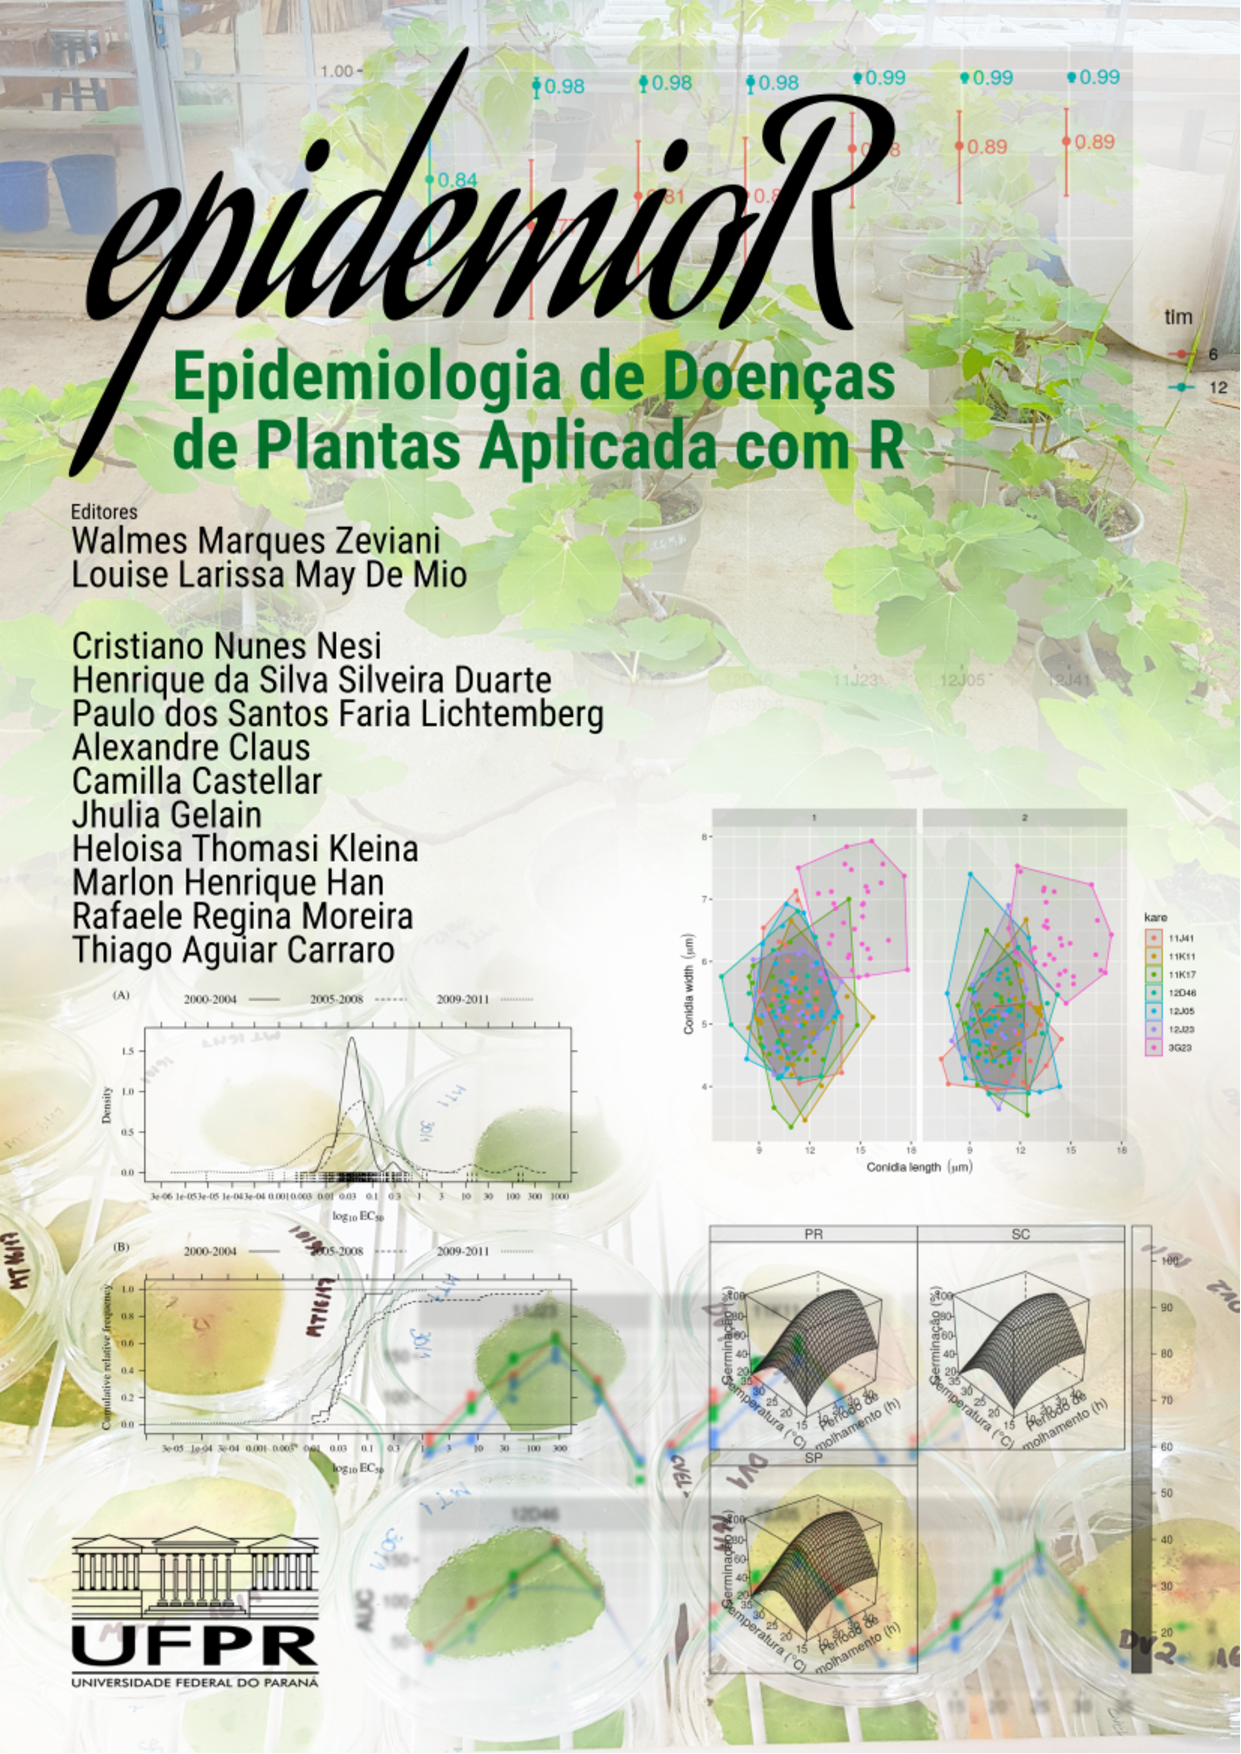
\includepdf{config/frontcover.pdf}

%~ %~ \maketitle
%~ 
% ---- CAPA ----

\begin{titlepage}
\thispagestyle{empty}
\centering

\topskip0pt
\vspace*{\fill}

% XX ABC - Congresso Brasileiro de Coisas
% \vspace{0.5cm}

\noindent\rule{\textwidth}{0.2mm}
% \vspace*{-0.5cm}

% Curso\\[0.2cm]

{\Large \textbf{\thetitle}}\\


% \vspace{0.25cm}
\noindent\rule{\textwidth}{0.2mm}
\vspace{0.5cm}

\thedate
\vspace{1.5cm}

\theauthor

\vspace*{\fill}
\end{titlepage}

\thispagestyle{empty}
\cleardoublepage

% ---- CAPA ----
% ---- Autores com informações ----

\thispagestyle{empty}
\cleardoublepage
\thispagestyle{empty}

\topskip0pt

\begin{flushleft}
{\Large \textbf{\thetitle}}\\

\end{flushleft}
\vspace*{1.5em}

\begin{flushleft}
            {\large Walmes Marques Zeviani}
      \newline {\footnotesize \faInstitution~~}Departamento de Estatística · UFPR
            \newline \faEnvelopeSquare~      \texttt{\href{mailto:walmes@ufpr.br}{\nolinkurl{walmes@ufpr.br}}}     
              \newline \faGlobe~                       leg.ufpr.br/\textasciitilde{}walmes        
      
      

         \vspace{1em}
            {\large Louise Larissa May De Mio}
      \newline {\footnotesize \faInstitution~~}Departamento de Fitotecnia e Fitossanidade · UFPR
            \newline \faEnvelopeSquare~      \texttt{\href{mailto:maydemio@ufpr.br}{\nolinkurl{maydemio@ufpr.br}}}     
              \newline \faGlobe~                       \url{http://www.agrarias.ufpr.br/portal/fitotecnia/louise-larissa-may-de-mio/}        
      
      

        \end{flushleft}

% ---- Autores com informações ----

\vspace*{2em}

\begin{flushleft} Laboratório de Estatística e Geoinformação (LEG)\\ \url{http://www.leg.ufpr.br}\\ Laboratório de Epidemiologia para Manejo Integrado de Doenças de Plantas (LEMID)\\ \url{http://www.lemid.ufpr.br/}\\ Universidade Federal do Paraná (UFPR)\newline\newline \end{flushleft}

\vspace*{\fill}

\begin{center} Curitiba, Paraná, Brasil\\ \the\year\\ \end{center}

\clearpage


{
\hypersetup{linkcolor=black}
\setcounter{tocdepth}{1}
\tableofcontents
}
\chapter*{Apresentação}\label{apresentacao}
\addcontentsline{toc}{chapter}{Apresentação}

O objetivo do \texttt{epidemioR} é fazer a documentação do uso do
software R no desenvolvimento, aplicação e avaliação métodos para
análise de dados em epidemiologia para manejo de doenças em plantas com
temas específicos de interesse dos professores, pesquisadores e alunos.

De forma geral, são vistas abordagens de análise que vão da aplicação do
R para análise de progresso temporal e espacial de doenças, estudo de
dispersão de inóculo, modelagem e previsão de epidemias, análises
multivariadas, análise de regressão múltipla e regressão não linear,
dentre outros conforme demanda. Procura-se, sem que haja distanciamento
dos objetivos da pesquisa, inovar no emprego de métodos estatísticos
para que haja melhor aproveitamento dos dados, o que se consegue
principalmente com: apropriadas visualizações gráficas, métodos de
análise contemporâneos e apropriados às características da investigação
e produção de código aberto e reproduzível.

A ênfase do curso é sobre problemas, delineamentos e abordagens de
análise comuns à área epidemiológica como aqueles com medidas repetidas
no tempo e experimentos realizados em vários anos e locais, também
àqueles que avaliem tempo até um desfecho (inoculação, esporulação),
dados de proporção (germinação, etc), dados de curva de crescimento
(modelos não lineares) e análise de dados de avaliação de doença
(incidência e severidade).

Este material é produzido devido à colaboração de professores e alunos
do Programa de Pós Graduação em Produção Vegetal, com colaboração de
professores e pesquisadores externos.

\chapter{Análise de sobrevivência}\label{analise-de-sobrevivencia}

\pagestyle{fancy}

\begin{flushright}
Camilla Castellar
\end{flushright}

\vspace{2em}

\section{Introdução}\label{introducao}

Espécies do gênero \emph{Colletotrichum} estão associadas a duas doenças
da macieira, denominadas de mancha foliar de Glomerella (MFG) e podridão
amarga (PA) \citep{Damm2012, Gonzlez2006}. A MFG causa sintomas em
folhas e diminutas lesões em frutos de macieira Gala, que não evoluem em
tamanho, enquanto a PA desenvolve podridões que podem cobrir toda a
superfície dos frutos. A relação entre os sintomas não é esclarecida
\citep{Kat2000} e algumas das hipóteses para os dois tipos de sintomas
associadas a um mesmo gênero são: o momento de infecção do patógeno,
presença de ferimentos nos frutos e espécie associada. Assim, o objetivo
do trabalho foi investigar os sintomas produzidos pelo patógeno
considerando as hipóteses destacadas anteriormente.

Dois experimentos semelhantes foram realizados com as cultivares Eva e
Gala. Frutos de cinco estágios fenologicos foram coletados no campo de
forma aleatória e mantidos em potes com umidade. Os frutos foram
inoculados com as espécies \emph{C. nymphaeae} e \emph{C. fructicola} em
maças com e sem ferimento. O delineamento experimental foi inteiramente
ao acaso em esquema de fatorial triplo, com 5 estágios fenológicos x 3
tipos de inoculação (2 espécies e a testemunha) x 2 formas de infecção
(com e sem ferimento) x 4 repetições. Cada repetição foi composta por 2
frutos mantidos em um mesmo pote e o experimento foi repetido em duas
áreas de coleta. As avaliações foram realizadas diariamente a partir da
inoculação e o tipo de sintoma foi associado a números. O número 0
corresponde ausência de sintomas, 1 sintomas de MFG, 2 para sintomas de
PA e 3 para lesões com esporulação nas lesões de PA (Figura
\ref{fig:sintomas}).





\begin{figure}

{\centering 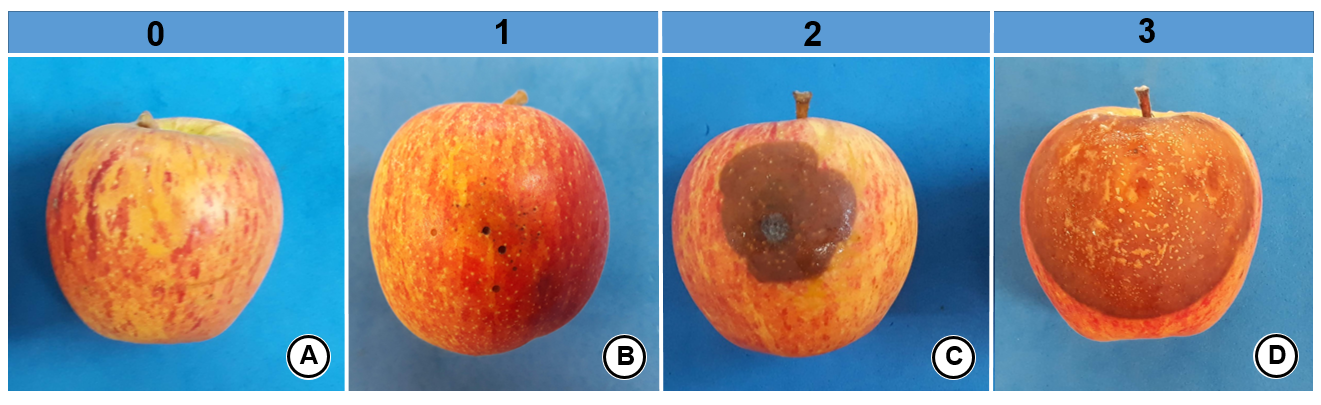
\includegraphics[width=1\linewidth]{./camilla/sintomas} 

}

\caption{Frutos de macieira sem sintomas (A), com mancha foliar de
glomerella em frutos (B), podridão amarga (C), lesão da podridão amarga
esporulando (D) e seus números correspondentes nas avaliações.}\label{fig:sintomas}
\end{figure}

\chapter{Germinação de ascósporos e conídios e Monociclo em
frutos}\label{germinacao-de-ascosporos-e-conidios-e-monociclo-em-frutos}

\section{Motivação}\label{motivacao}

O Cancro Europeu das Pomáceas e Podridão de frutos causados por
\emph{Neonectria ditissima} ocorre em regiões produtoras de maçãs
(\emph{Malus domestica} Borkh.) do mundo todo, como Europa, América do
Norte, Chile, Austrália, Nova Zelândia, Japão e África do Sul
\citep{Beresford2011}. Detectada no Brasil em 2002, se destaca entre as
doenças que vêm causando grandes perdas na cadeia produtiva da macieira.
A doença afeta os ramos e o tronco principal da planta causando sintoma
de cancro, enquanto em frutos causa podridão mole (Figura
\ref{fig:prancha01}). A podridão de Neonectria em frutos de maçã ocorre
na maioria das áreas produtoras do mundo, e no Brasil sua elevada
incidência pode ser explicada pelas condições climáticas mais favoráveis
e/ou pela maior quantidade de inóculo nos pomares, devido à falta de
experiência no manejo \citep{EmbrapaCancro2015}.




\begin{figure}

{\centering 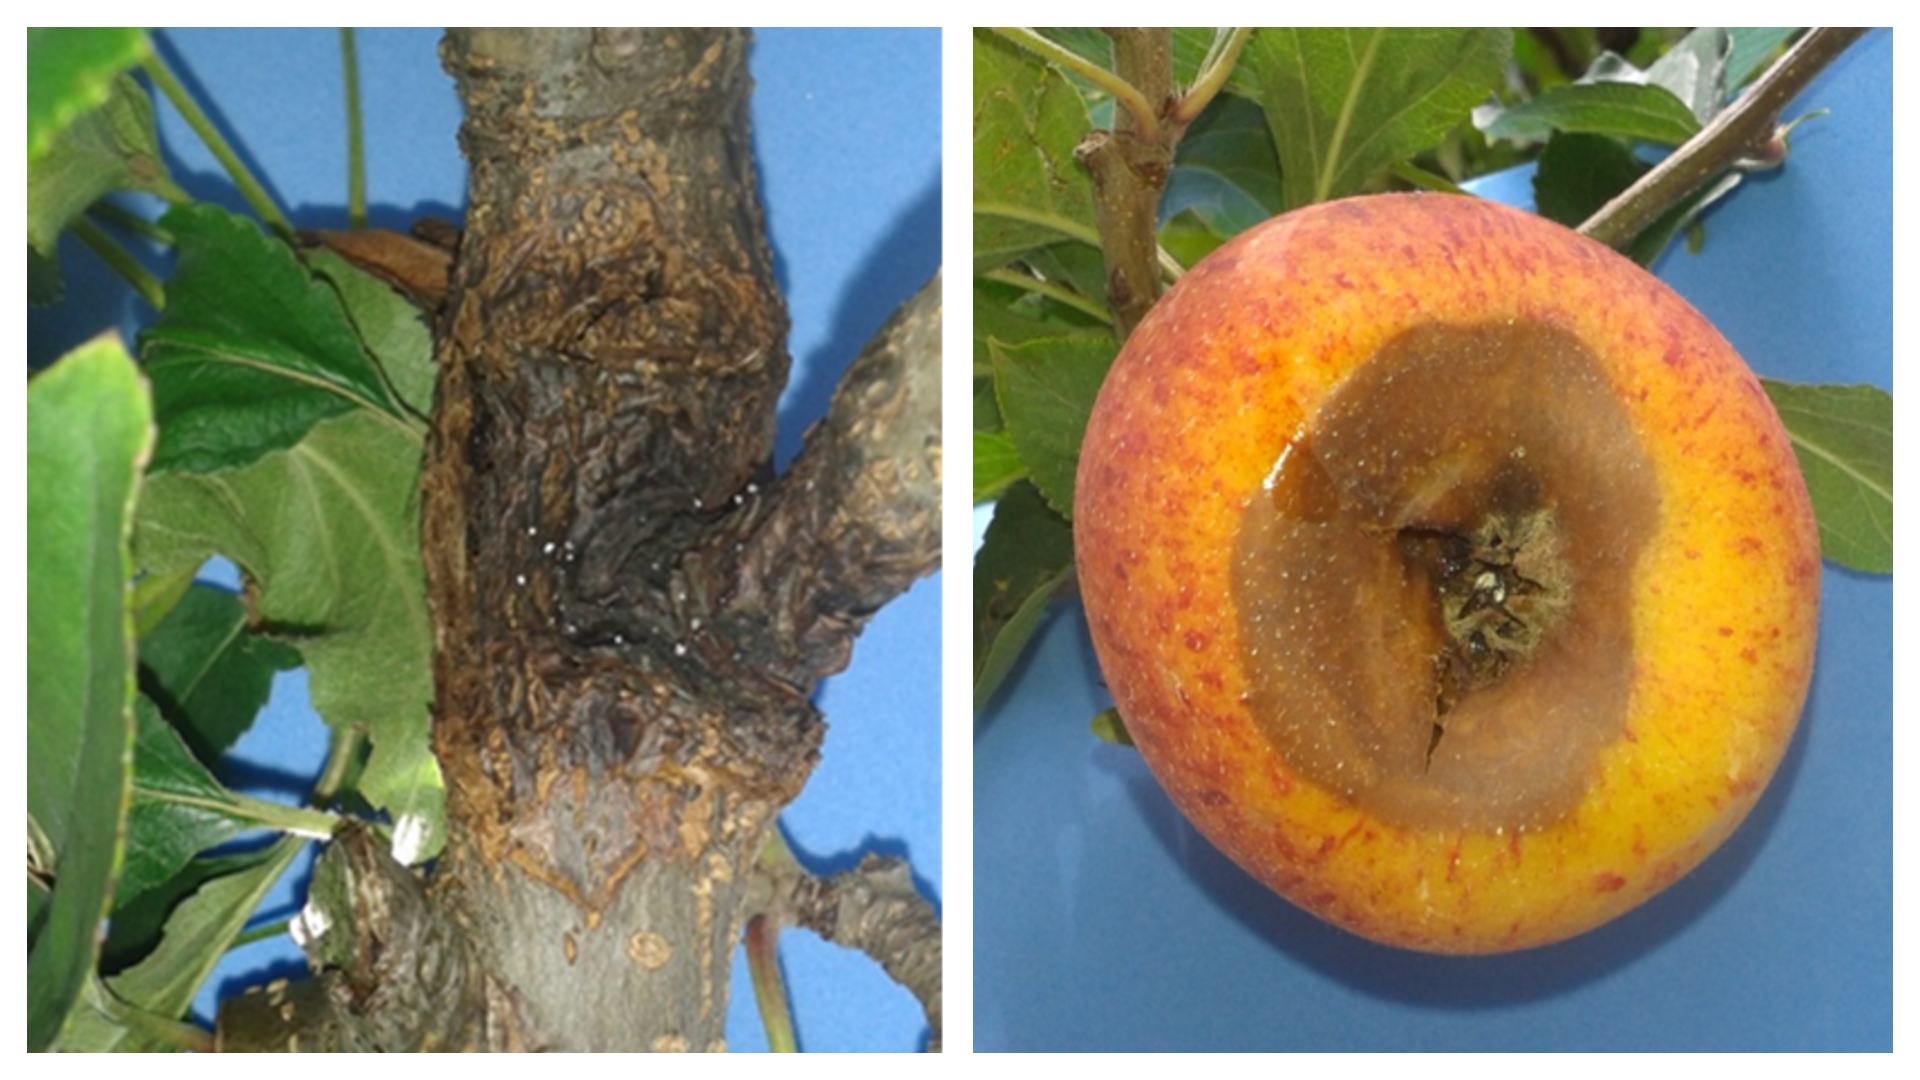
\includegraphics[width=1\linewidth]{./jhulia/prancha01} 

}

\caption{Sintomas de Cancro Europeu em macieira (esq.) e de
podridão de Neonectria em fruto (dir.) em cultivar Gala.}\label{fig:prancha01}
\end{figure}

O fungo produz dois tipos de esporos, sendo os ascósporos produzidos
sexuadamente em peritécios e os conídios produzidos assexuadamente em
esporodóquios (Figura \ref{fig:prancha02}). Os dados disponíveis sobre
as taxas de germinação de ascósporos em diferentes temperaturas vão até
um período de oito horas \citep{Latorre2002} e devem ser complementados.
A comparação entre a germinação de ascósporos e conídios em diferentes
temperaturas e períodos de incubação é relevante para a predição de
riscos de acordo com o esporo predominante no pomar.




\begin{figure}

{\centering 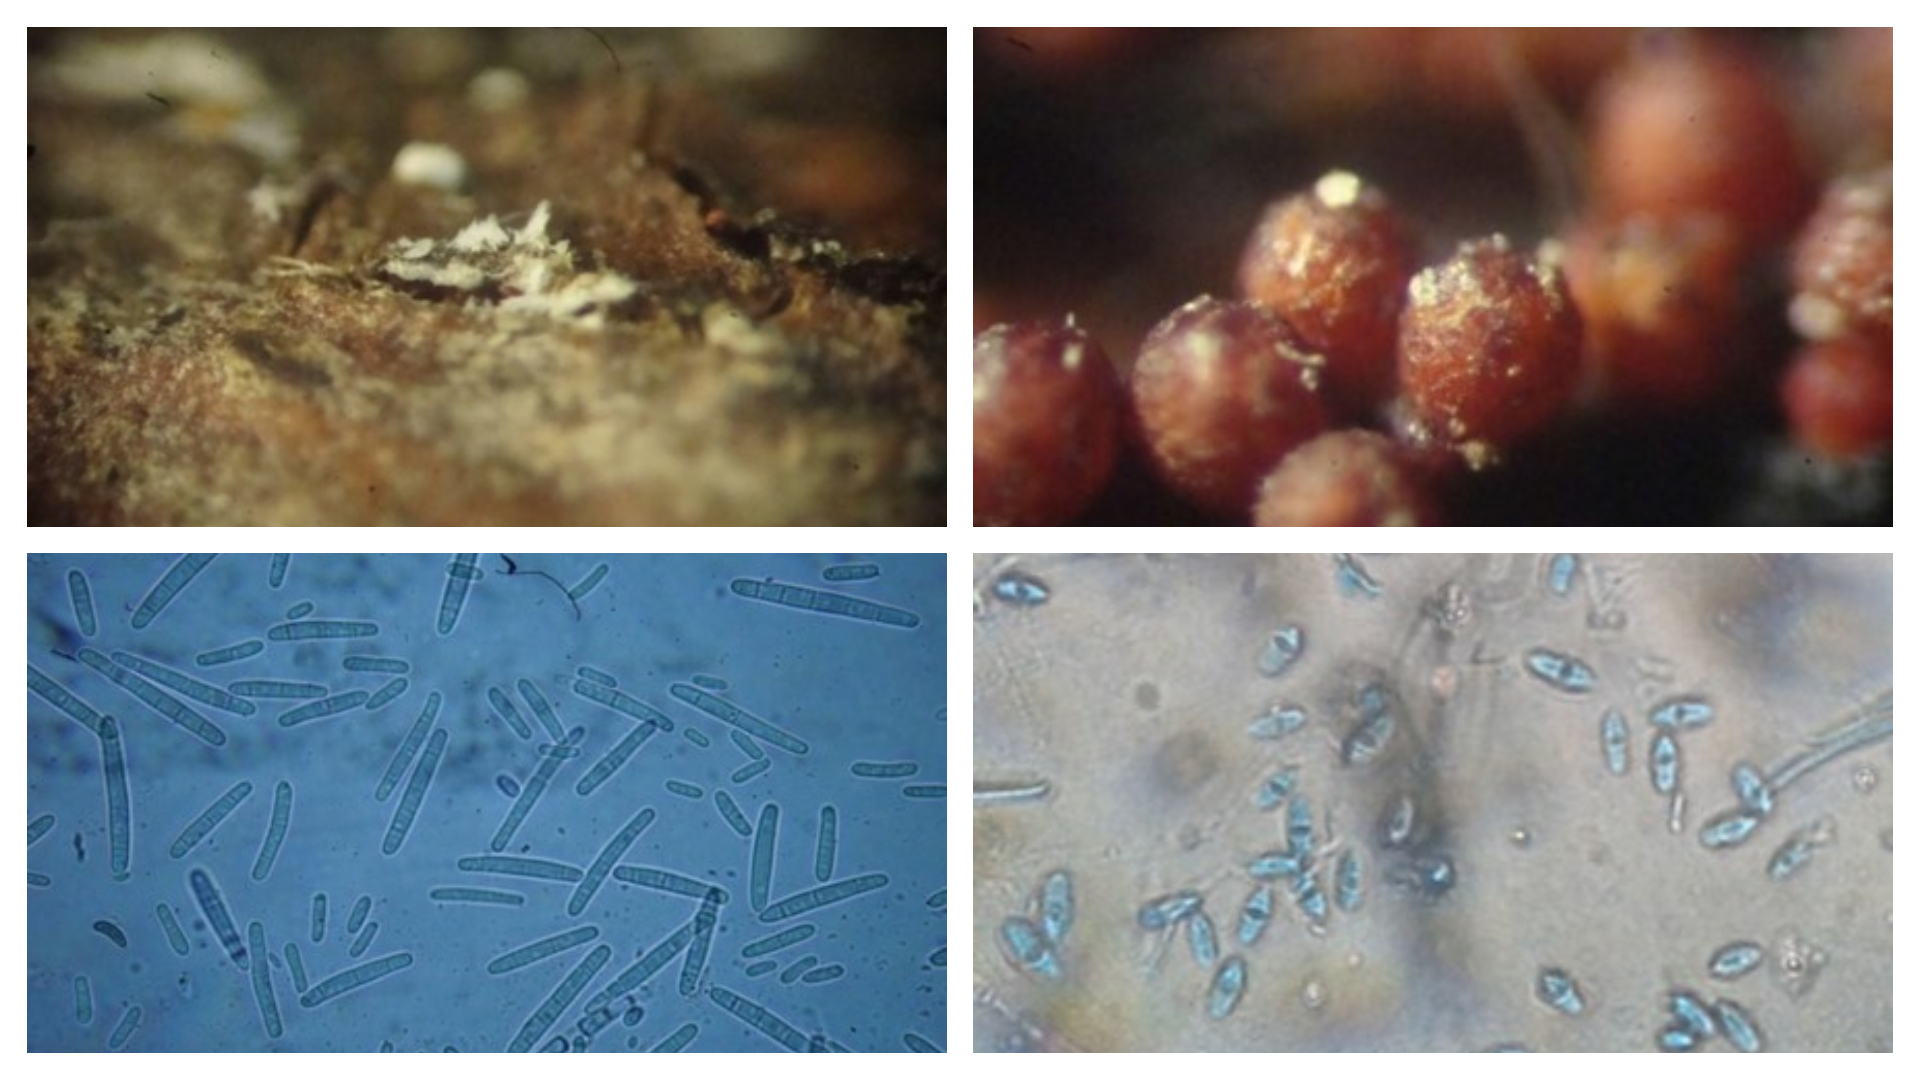
\includegraphics[width=1\linewidth]{./jhulia/prancha02} 

}

\caption{Esporodóquio produzindo conídios (esq.) e peritécios
produzindo ascósporos (dir.) de \emph{Neonectria ditissima}.}\label{fig:prancha02}
\end{figure}

Embora \emph{N. ditissima} seja mais comumente descrito como patógeno da
macieira, a pera (\emph{Pyrus communis} L.) também é hospedeira
\citep{Flack1977} e, ocasionalmente, os pomares de pera apresentam alta
incidência da doença \citep{Weber2014}. Os pomares de pera são comumente
plantados próximos aos pomares de maçã devido à semelhança entre os
requisitos de horas de frio e tratamentos culturais, o que pode
representar risco caso a doença chegue aos pomares de pereira e estes
sejam suscetíveis. Não há nenhum relato científico recente sobre a
podridão de frutos por Neonectria sobre pera, e o monociclo da doença
nesse fruto nunca foi elucidado.

Esse capítulo objetivou a elucidação e comparação de modelos polinomial
e beta-monomolecular para avaliação de dados de germinação de conídios e
ascósporos em diferentes temperaturas e períodos de molhamento, bem como
descrever equações que descrevam o comportamento do monociclo da
podridão de Neonectria em frutos de pera e maçã.

\section{Germinação de conídios e
ascósporos}\label{germinacao-de-conidios-e-ascosporos}

Temperaturas de 12 a 35 graus com períodos de incubação de 3 a 60 horas.

A Tabela \ref{tab:germinacao-neonectria-ditissima} descreve como os
dados da germinação de \emph{Neonectria ditissima} foram tabulados.





\begin{table}[t]

\caption{\label{tab:germinacao-neonectria-ditissima}Descrição do tipo de esporo
(ascósporo ou conídio), temperatura (°C), período de incubação (h) e
germinação (\%).}
\centering
\begin{tabular}{ccccc|ccccc|ccccc|ccccc|ccccc}
\hline
Sepal.Length & Sepal.Width & Petal.Length & Petal.Width & Species\\
\hline
NA & 4 & 1 & 0.2 & setosa\\
\hline
NA & 3 & 1 & 0.2 & setosa\\
\hline
NA & 3 & 1 & 0.2 & setosa\\
\hline
NA & 3 & 2 & 0.2 & setosa\\
\hline
NA & 4 & 1 & 0.2 & setosa\\
\hline
NA & 4 & 2 & 0.4 & setosa\\
\hline
\end{tabular}
\end{table}

\chapter{Antracnose do Caquizeiro}\label{antracnose-do-caquizeiro}

\pagestyle{fancy}

\begin{flushright}
Thiago de Aguiar Carraro\\
Paulo dos Santos Faria Lichtemberg\\
Walmes Marques Zeviani\\
Louise Larissa May De Mio
\end{flushright}

\vspace{2em}

O caqui (\emph{Diospyros kaki}) é uma fruta de alto valor nutricional e
se aclimata muito bem em regiões de clima temperado e subtropical. O
Brasil, é o quinto maior produtor e sua produção está concentrada nos
estados de São Paulo, Rio Grande do Sul, Paraná e Minas Gerais
\citep{fao2017}. Nos últimos anos, a produção de caqui vem sofrendo uma
grande queda da produção, decorrente em parte, da antracnose.

A antracnose, causada por \emph{Colletotrichum} spp., é uma doença
severa que pode infectar ramos, folhas e frutos, ocasionando sérios
danos aos produtores, devido a queda prematura dos frutos. O principal
agente causal é o fungo \emph{Colletotrichum horii}, entretanto
recentemente foram relatadas outras espécies patôgenicas ao caquizeiro
\citep{maydemio2015, blood2015}. As espécies \emph{C. fructicola},
\emph{C. nymphaeae} e \emph{C. melonis} foram relatadas também como
causadores de antracnose em caquizeiro no Brasil \citep{carraro2019}
(Figura \ref{fig:prancha-1}).






\begin{figure}

{\centering 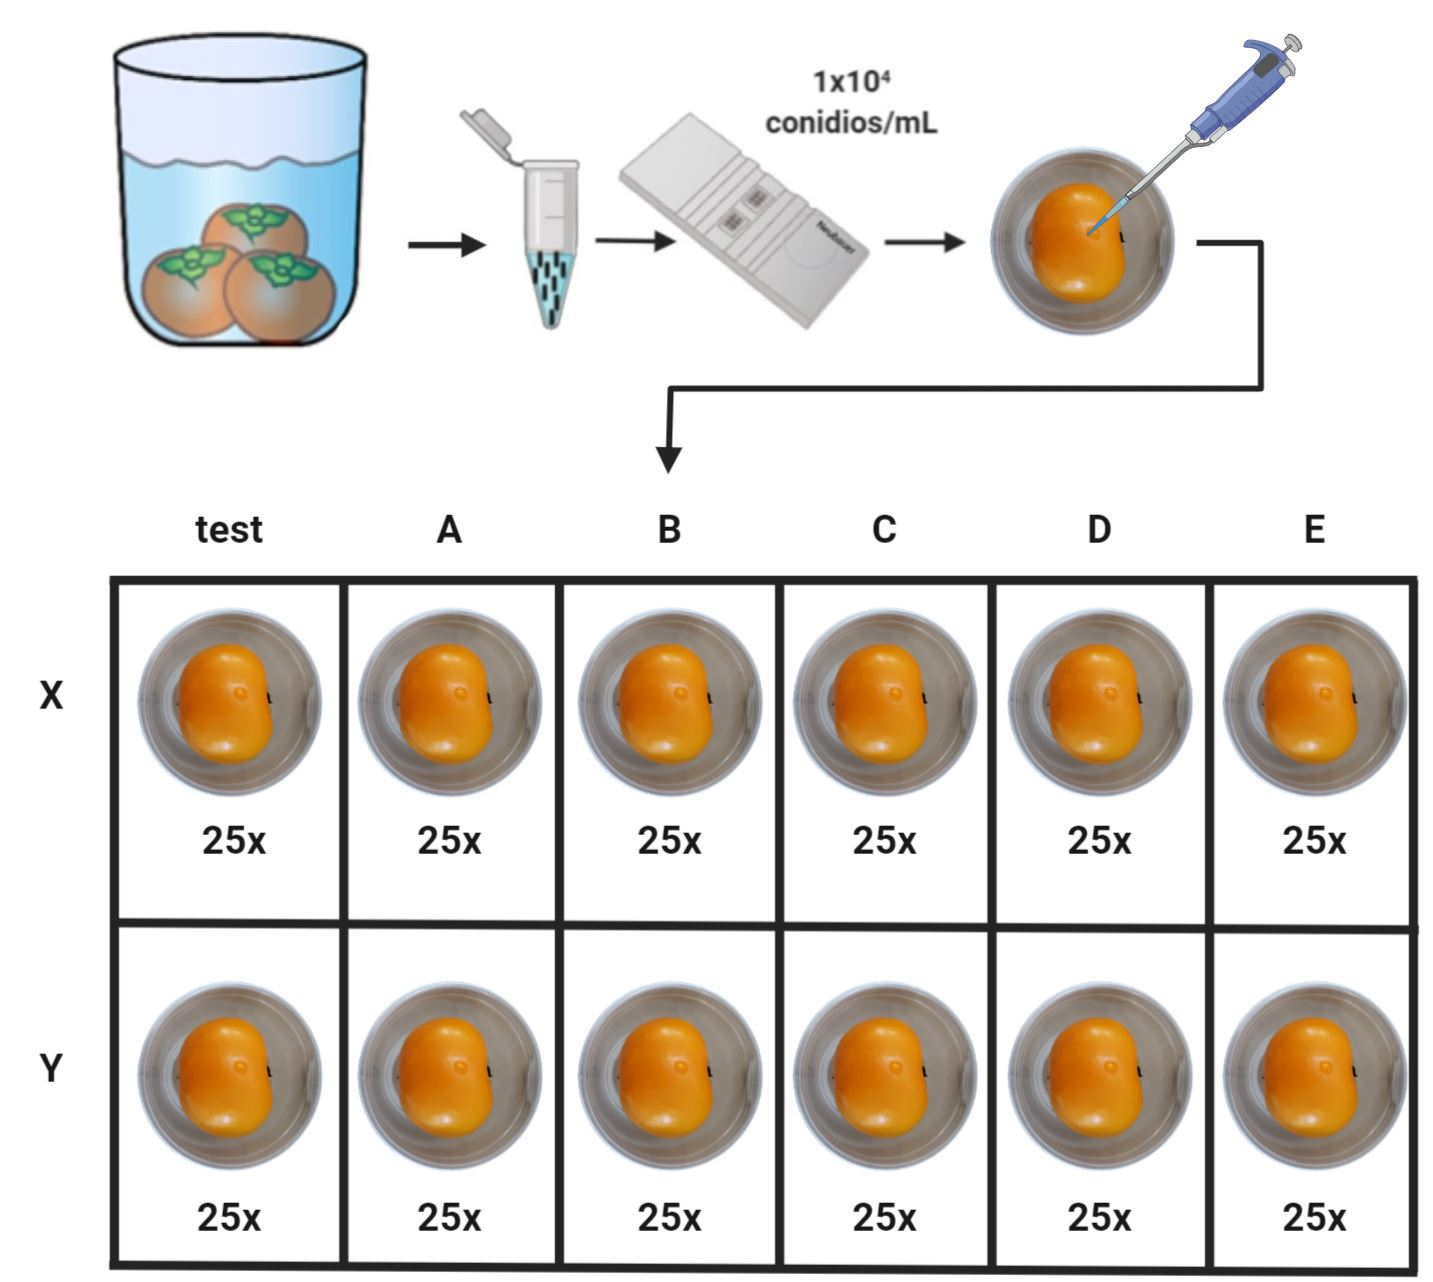
\includegraphics[width=1\linewidth]{./tac/prancha_1} 

}

\caption{Lesões necróticas, deprimidas, escuras e circulares em
frutos imaturos (massa de conídios em detalhe) (A) e maduros (B) de
caquizeiro. Lesões de antracnose (C) e esporulação em ramos jovens (D) e
em folhas (E). Queda prematura dos frutos (F)}\label{fig:prancha-1}
\end{figure}

O controle químico é uma das formas mais eficientes para o controle de
doenças de plantas, porém para o caquizeiro tem-se poucos produtos
registrados no Brasil, dentre estes produtos mais de 60\% apresentam
riscos de médio a alto para o desenvolvimento de resistências do fungo à
fungicidas (DMI e QoI) e, consequentemente podem resultar em uma perda
da eficiência em campo, caso os mesmos não sejam adequadamente
manejados. Para adotar estratégias de controle eficientes ao longo das
safras é necessário que seja realizado o monitoramento da sensibilidade
do fungo aos fungicidas.

Em estudos iniciais de monitoramento da sensibilidade de
\emph{Colletotrichum} spp. aos fungicidas registrados para o caquizeiro,
foi observado uma sensibilidade alterada para os ingredientes ativos dos
grupos QoI e DMI, os quais ainda nem estão registrados para antracnose,
apenas para cercosporiose. Além disso, na coleção de isolados de
\emph{Colletotrichum} spp. do LEMID, obtido de caquizeiro, foi observada
diferenças na eficiência dos fungicidas em relação às espécies
relatadas, o que implicará no manejo dependendo da espécie preponderante
em cada região (dados ainda não publicados). Estes resultados demonstram
a importância dos programas de pulverizações considerando sensibilidade
inerente e eficiência dos fungicidas. Somado a isso, o manejo de número
de aplicações por safra alternando grupos químicos e incluindo
fungicidas de amplo espectro são importantes para evitar sobreposição de
populações menos sensíveis, o que dificultará no manejo da doença.

\section{\texorpdfstring{Metodologias para monitoramento da
sensibilidade do fungo à fungicidas (\emph{in vitro}) e Ensaio para
teste de eficiência dos fungicidas (\emph{ex
vivo})}{Metodologias para monitoramento da sensibilidade do fungo à fungicidas (in vitro) e Ensaio para teste de eficiência dos fungicidas (ex vivo)}}\label{metodologias-para-monitoramento-da-sensibilidade-do-fungo-a-fungicidas-in-vitro-e-ensaio-para-teste-de-eficiencia-dos-fungicidas-ex-vivo}

A alteração da sensibilidade do fungo a um fungicida pode ser monitorada
\emph{in vitro} antes que ocorra uma falha no controle da doença em
campo \citep{yuan2013}. Diante disso, ensaios de CE\textsubscript{50} e
de dose discriminatória são importantes para observação dessa mudança de
sensibilidade. A CE\textsubscript{50} mostra curvas de dose-resposta que
são possíveis estimar a concentração efetiva capaz de inibir 50\% do
diâmetro micelial ou da germinação dos esporos do fungo e , com os
valores de CE\textsubscript{50} de diferentes isolados e de diferentes
anos é possível comparar se esta ocorrendo uma mudança de sensibilidade,
assim possibilitará adotar estatrégias para o controle da doença
\citep{forster2004}.

O método da dose discriminatória é muito utilizado pela sua praticidade
e rapidez em obtenção de uma resposta exploratória da sensibilidade de
uma população de isolados, devido a redução de unidades experimentais
\citep{lichtemberg2016}. Este método inclui o uso de uma única dose que
pode determinar se um isolado é resistente ou sensível \citep{russell}.

Os experimentos de dose-resposta por avaliação de diâmetro micelial ou
germinação dos esporos são geralmente realizados em diferentes placas de
Petri contendo diferentes concentrações de fungicidas difusos no meio de
cultura. Há variações das técnicas, como a diluição em gradiente
espiral, na qual \emph{M. fructicola} foi um dos patógenos utilizados
para validar o método com diferentes fungicidas: diclorana, fludioxonil,
fenehexamida e tebuconazol \citep{forster2004}. Para esse método,
diferentes concentrações de fungicidas são distribuídas em espiral numa
mesma placa formando um gradiente de concentrações, no qual no centro há
as maiores concentrações e nos bordos as menores. Esporos do patógeno
são incubados em tiras de palito de madeira autoclavados ou em meio de
cultura e, quando apresentarem crescimento micelial uniforme, essas
tiras são transferidas para as placas com e sem fungicida, de forma que
o fungo esteja em contato com todas as diferentes concentrações.
Comparando com o crescimento do fungo a partir da tira no meio sem
fungicida, com esta técnica é possível determinar a concentração efetiva
capaz de inibir 50\% do diâmetro micelial de uma forma mais rápida,
econômica e precisa \citep{forster2004, amiri2014}.

Além desses métodos, ensaios \emph{ex vivo} são também muito relevantes
para determinar se esta ocorrendo um resistência prática, ou seja,
quando ocorre uma falha do controle da doença em campo
\citep{ghinirekimatih2000}. Estes testes podem ser realizados com
plantas ou partes vegetais destacados, o qual serão tratados com a
concentração recomendada para o produtor.

\chapter{Motivação}\label{motivacao-1}

\section{Phakopsora pachyrizi}\label{phakopsora-pachyrizi}

A soja, \emph{Glycine max} (L.) Merr, é uma das commodities mais
importantes a nível mundial, pois é fonte de óleo e proteína para
alimentação humana e animal \citep{conab}. A produtividade dessa cultura
pode ser afetada por doenças, principalmente a ferrugem asiática causada
pelo fungo \emph{P. pachyrhizi}.

O manejo da ferrugem asiática é executado principalmente com o uso de
fungicidas do grupo dos inibidores de desmetilação (IDM's), inibidores
de quinona externa (IQe's), inibidores da succinato desidrogenase
(ISDH's) e o tradicional mancozebe. Falhas no controle da ferrugem da
soja tem sido observada nos últimos anos em diferentes regiões do
Brasil, devido a mutações do fungo \citep{godoy2019}.

Foi relatado mutações em isolados de \emph{P. pachyrhizi} nos genes
cyp51 \citep{schmitz2013}, cytb \citep{klosowski2015} e sdh-c
\citep{simoes2017}. Genótipos com resistência nos genes cyp51 e cytb são
mais comumente encontrados \citep{klosowski2016} porém recentemente foi
descrito a ocorrência de múltipla resistência para estes três genes no
mesmo isolado \citep{muller}.

Frequentemente, isolados resistentes a fungicidas são menos adaptados,
se comparado com isolados sensíveis. Evidências experimentais sobre
estudo de adaptabilidade sugerem que isso ocorre com isolados mutantes
que têm resistência a fungicidas do grupo dos Qoi \citep{klosowski2016}.

Entretanto, pouco se sabe sobre a estabilidade e adaptabilidade da
mutação no gene SDH-c que confere resistência aos fungicidas do grupo
SDHI. Assim como, quanto ao comportamento epidemiológico de populações
de diferentes regiões do Brasil, nas diferentes condições ambientais.
Desta forma, serão conduzidos ensaios visando conhecer melhor a dinâmica
populacional de P. pachyrhizi oriundas de diferentes localidades do
Brasil e, isolados destas populações.

Neste trabalho será abordado analises estatisticas com o uso do R, para
alguns dos componentes de adaptabilidade das populações \emph{P.
pachyrhizi} oriundas de diferentes regiões produtoras do Brasil. Será
analisado os parâmetros de monociclo em plantas e folha destacada em
diferentes condições de temperatura; a germinação de esporos em
diferentes tempo de exposição a radiação UV; em diferentes temperaturas
e incidencia luminosidade; a germinacao em meio salino e quanto ao
stress oxidativo das populacoes. Para tal se utilizou seis populações.
Alem disso, será analisado a EC50 de alguns grupos quimicos de
fungicida.



\begin{figure}

{\centering 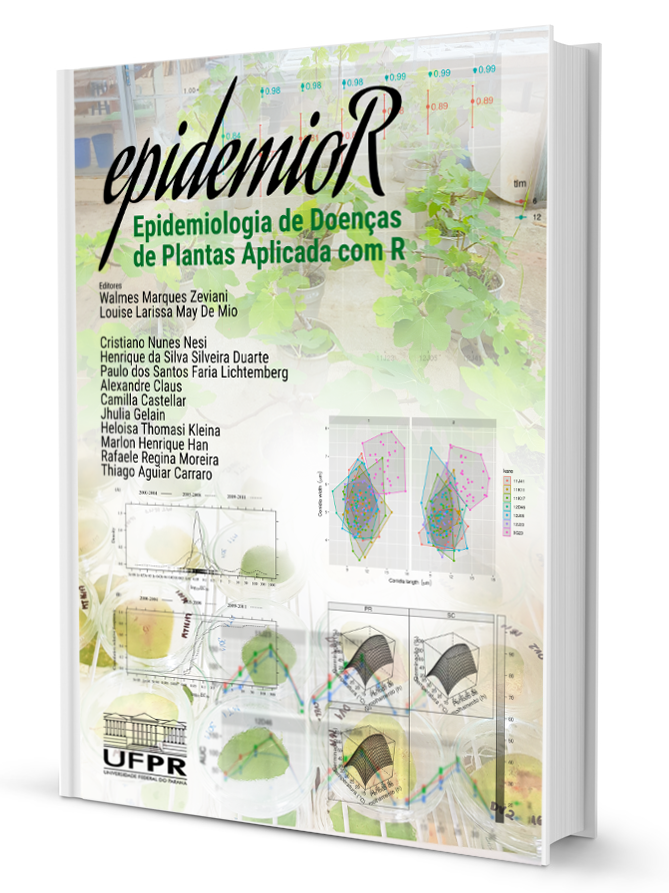
\includegraphics[width=1\linewidth]{./config/bookcover} 

}

\caption{Escala diagramática.}\label{fig:image1}
\end{figure}

\bibliography{config/refs.bib,jhulia/refs.bib,camilla/refs.bib,tac/refs.bib,alexandre/refs.bib}


\end{document}
